%---------------------------------------------------------------------------------------------------
% Realization
%---------------------------------------------------------------------------------------------------
\newpage
%\part{Anfang}
\chapter{Realization}\label{cap:Realization}
\subsection{Application Class}
An Application Class is called before the MainActivity is called for the first time. Due to the usage of Backendless (BaaS) the applicationId, Api Key and the serverUrl are stored in the ApplicationClass and connects the Webapplication with the Android Application. It also contains variables for the user credentials saved in the Backendless.user table and the Artefact table. 

\subsection{Backendless}
Backendless provides the server data to the app when it is requested. This happens in case of registration, login, artefact creation, file upload, file download, geolocating marker, edit artefact, etc.
Independently which data is needed, an asynchronous Backendless request requires the implemention of two interface methods. The asyncCallback methods "handleResponse()" and "handleFault()" are recommended to keep the main thread free and increasing the application performance. "handleFault()" is called if something went wrong. "handleResponse()" is called if the request was successful and provides the requested data.

\subsubsection{User table}
With Backendless one can create data tables with ease. The user table should contain certain properties such as name, email and password. To get a table like that one calls the Backendless.UserService.register() and pass a BackendlessUser object as argument.

An exemplary interaction between app and backendless is displayed here in case of user registration.

\fbox{
\lstinputlisting[label={code:backendless_register} ,caption={Backendless user registration},captionpos=b, language = java,  numbers = left]{program/backendless_register.java}
}

The method handleResponse() returns to the LoginFragment, waiting for the user to login. From now on the user table is listed within the Backendless console (Webapplication) \ref{fig:backendlessConsoleUserTable}.


\subsubsection{LoginFragment}
This Fragment is the first view which appears to the user. It provides three possibilities. 
\begin{itemize}
\item Login
\item Register
\item Password recovery
\end{itemize}
The first step for a new user is moving to the RegisterFragment via button click.
If the registration is accomplished, one can login or reset password.
Successful login leads to the Map, which is the main part of the application. It keeps the user logged in until the logout button is clicked, hence the next time Civitas is started it navigates directly to the Map.

The Login progress is displayed here. 

\fbox{
\lstinputlisting[label={code:backendless_login} ,caption={Backendless user login},captionpos=b, language = java,  numbers = left]{program/backendless_login.java}
}

A basic Backendless request implements two methods, handleResponse() and handleFault(). If request is successful, the response contains the user data. This data is stored in the Applicationclass.user for further purpose.

\subsubsection{User table}
The user table contains the same properties like the BackendlessUser object \ref{code:backendless_register} where it is created from plus the properties \textit{created} and \textit{updated} which where provided automatically from the Backendless.

\begin{figure}[H]
	\centering 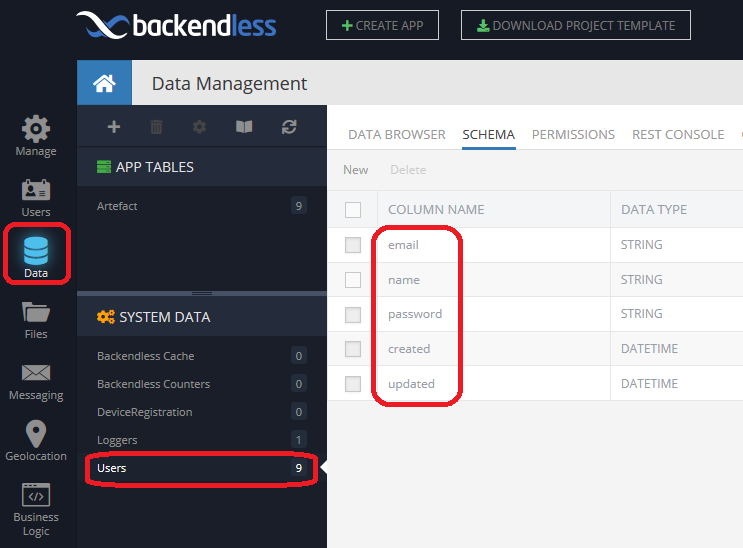
\includegraphics[width=0.8\textwidth]{backendless_console_user_table.png}
	\caption[backendlessConsoleUserTable]{Backendless console user table}
	\label{fig:backendlessConsoleUserTable}
\end{figure}
\footnotetext{URL: https://www.banksy.org [cited 22 August 2018]}


ich realisiere!